\documentclass[8pt]{beamer}

% handout
% \documentclass[handout, 10pt]{beamer}

\usepackage{clases}

\title{Investigación Operativa}
\subtitle{Ciclos Hamiltonianos/Eulerianos - Planaridad}
\date{}
\author{Facundo Gutiérrez - Nazareno Faillace}
\institute{Departamento de Matemática, FCEN, UBA}
% \titlegraphic{\hfill\includegraphics[height=1.5cm]{logo.pdf}}

\newcommand \anchoPagina{1.0} % El proyector no anda bien, hay que ajustar el ancho
\begin{document}

\maketitle

% \begin{frame}{Contenidos}
%   \setbeamertemplate{section in toc}[sections numbered]
%   \tableofcontents[hideallsubsections]
% \end{frame}

% \section{Introducción}
\section{Camino y Ciclo Euleriano/Hamiltoniano}

\begin{frame}{Camino y Ciclo Euleriano}
	\begin{minipage}{\anchoPagina \textwidth}
		Un \textit{camino euleriano} en un grafo $\mathcal{G}$ (o multigrafo en este caso, la definici\'on no cambia) es un camino que recorre todas las aristas de $\mathcal{G}$ exactamente una vez.
		\pause
		
		An\'alogamente, un \textit{circuito euleriano} es un circuito que recorre todas las aristas exactamente una vez.
		
		\textbf{Observaci\'on}: Si un grafo tiene m\'as de una componente conexa no trivial (que la componente no sea un v\'ertice aislado), entonces el grafo no tiene un circuito euleriano.
		\vspace{0.2cm}

	\end{minipage}
\end{frame}

\begin{frame}{Camino y Ciclo Euleriano}
	\begin{tcolorbox}[title=Teorema]
		Sea $\mathcal{G} = (\mathbb{V},\mathbb{E})$ conexo. Son equivalentes:
		\begin{enumerate}
			\item $\mathcal{G}$ tiene un circuito euleriano.
			\item Todo v\'ertice $v\in \mathbb{V}$ tiene grado par.
		\end{enumerate} 
	\end{tcolorbox}
	
	$(1 \Rightarrow 2)$ Sea $P$ un circuito euleriano en $\mathcal{G}$. Para cada vértice $v$ en la secuencia de $P$, se recorren las aristas ${u,v}$ y ${v,w}$, siendo $u$ y $w$ los vértices que anteceden y preceden a $v$ en $P$, respectivamente. Al ser euleriano, el circuito $P$ utiliza cada arista exactamente una vez y por lo tanto el grado de cada vértice debe ser par.

    
\end{frame}

\begin{frame}{Camino y Ciclo Euleriano}
    
    \begin{columns}
    \small
        \column{0.5\textwidth}
    	$(2 \Rightarrow 1)$ Supongamos que todos los vértices tienen grado par. Haremos inducción en $m$ la cantidad de aristas. Para $m=1$ y $m=2$ no existen grafos conexos cuyos vértices tengan todos grados par. Así que consideramos como caso base a $m=3$. En este caso, $\mathcal{G} = K_3$, que es claramente euleriano.
        \pause
        
        \vspace{1em}
    	Veamos el caso de un grafo con $m>3$ aristas cuyos vértices tienen todos grado par. Comenzamos con un vértice $v$ y elegimos una arista cualquiera que sea incidente a él. Desde el vecino de $v$ elegimos una arista incidente cualquiera que no hayamos utilizado. Y así sucesivamente hasta volver a $v$. Llamamos a este circuito $W$. Sabemos que existe tal circuito porque cada vez que visitamos un vértice distinto de $v$ estamos utilizando una arista adyacente. Como todo vértice tiene grado par, hay un número par de aristas adyacentes a cada vértice y siempre habrá alguna que no hayamos utilizado. Por lo tanto, con este proceso nos podemos construir un camino que nos lleve de vuelta a $v$.
    	\column{0.5\textwidth}
    	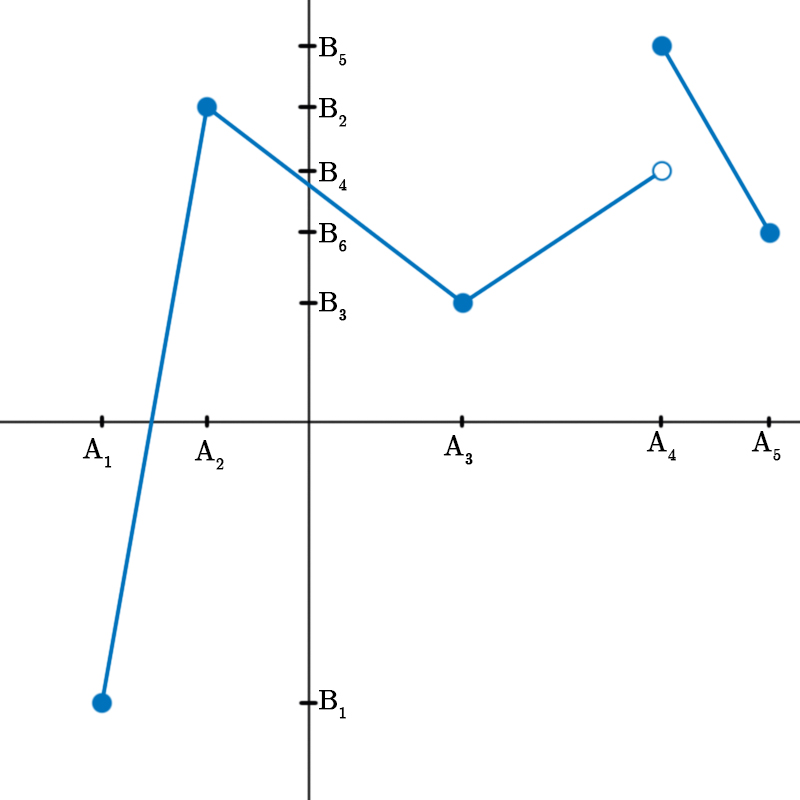
\includegraphics[width=\textwidth]{imagenes/g1.jpg}
    \end{columns}

\end{frame}

\begin{frame}{}
    \begin{columns}
    \small
        \column{0.5\textwidth}
    	Sean $E_W$ las aristas de $W$ y supongamos que $E_W\neq E$ (si no, ya tendríamos un circuito euleriano). El grafo $\mathcal{G}'$ que se obtiene de eliminar las aristas $E_W$ de $E$ tiene componentes conexas $C_1,\dots,C_k$. Cada una de estas componentes conexas cumple con la hipótesis inductiva: son  conexas, con menos de $m$ aristas y cada vértice tiene grado par. Esto último vale porque cuando eliminamos las aristas de $W$, removimos un número par de aristas incidentes en los vértices de $W$. \visible<2->{Por inducción, cada $C_i$ tiene un un circuito euleriano $E_i$.}
    	
	    \vspace{1em}
	    \visible<3->{Como $\mathcal{G}$ es conexo, hay un vértice $a_i$ de $C_i$ que se encuentra en $E_i$ y en $W$. Sin pérdida de generalidad, se puede asumir que a medida que recorremos $W$, se encuentra a $a_1,a_2,\dots,a_k$ en ese orden.}
	    
	    \vspace{1em}
	    \visible<4>{
	    Luego, obtenemos un circuito euleriano en $\mathcal{G}$ de la siguiente manera: comenzamos en $v$ y recorremos el circuito $W$ hasta llegar a $a_1$. Desde allí, recorremos $E_1$ hasta volver a $a_1$. Continuamos recorriendo $W$ hasta $a_2$ y desde allí se recorre $E_2$ hasta volver a $a_2$. Y así sucesivamente hasta alcanzar $a_k$, recorrer $E_k$ y desde $a_k$ volver a $v$ recorriendo $W$.}
    	\column{0.5\textwidth}
    	\visible<1-4>{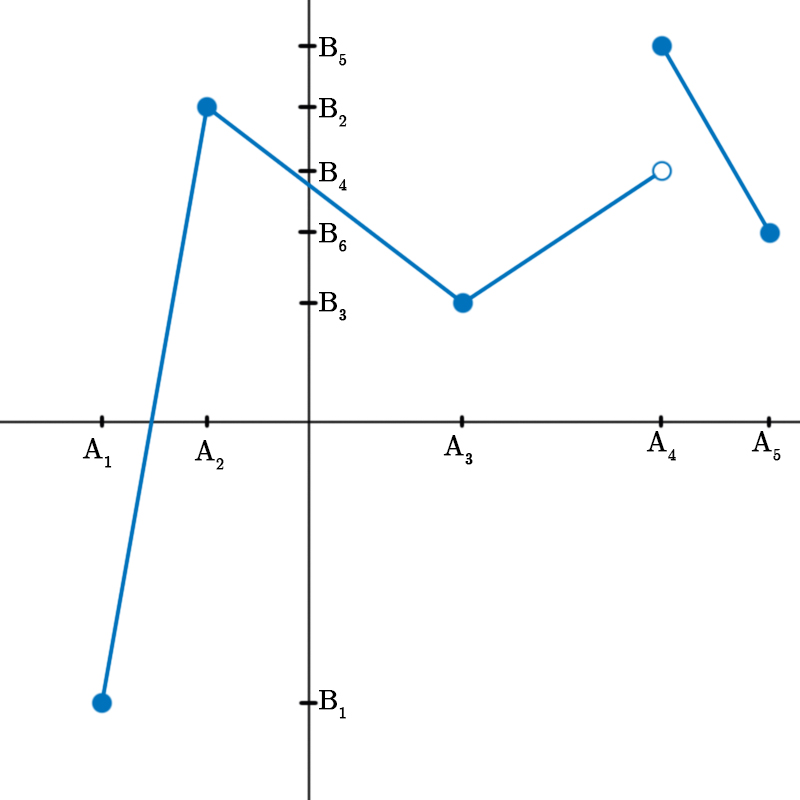
\includegraphics[width=\textwidth]{imagenes/g1.jpg}}
    \end{columns}

\end{frame}

\begin{frame}{Camino y Ciclo Euleriano}
    \begin{tcolorbox}[title=Corolario]
        Sea $\mathcal{G} = (\mathbb{V},\mathbb{E})$ un grafo conexo,
        
        $\mathcal{G}$ es euleriano $\iff$ $\mathbb{E}$ puede particionarse en circuitos.
    \end{tcolorbox}
    
\end{frame}

\begin{frame}{Camino y Ciclo Hamiltoniano}
	\begin{minipage}{\anchoPagina \textwidth}
		Un \textit{camino hamiltoniano} en un grafo $\mathcal{G}$ es un camino que recorre todos los v\'ertices de $\mathcal{G}$ exactamente una vez.
		\pause
		
		An\'alogamente, un \textit{circuito hamiltoniano} es un circuito que recorre todos los v\'ertices exactamente una vez.
		\pause
		
		\textbf{Observaci\'on}: Si un grafo no es conexo, entonces el grafo no tiene un circuito hamiltoniano.
		\pause
		\vspace{1em}
		\begin{tcolorbox}[title=Teorema de Dirac]
		    Si el grado de cada v\'ertice de un grafo conexo y simple es al menos $\frac{|\mathbb{V}|}{2}$, entonces existe un camino hamiltoniano.
		\end{tcolorbox}
		\pause
		\vspace{1em}
		\begin{tcolorbox}[title=Teorema de Ore]
		    Si la suma de los grados de cada par de v\'ertices no adyacentes de un grafo conexo y simple es al menos $|\mathbb{V}|$, entonces existe un camino hamiltoniano en el grafo.
		\end{tcolorbox}
		
	\end{minipage}
\end{frame}

\begin{frame}{Ejercicio 1}
		\begin{minipage}{\anchoPagina \textwidth}
				Llamemos $\phi(\mathcal{G})$ al n\'umero de componentes conexas de $\mathcal{G}$. Mostrar que si $\mathcal{G}$ es conexo no trivial y todos sus v\'ertices tienen grado par, entonces para cualquier v\'ertice $v$ se cumple que $\phi(\mathcal{G}\setminus \{v\}) \leq \frac{d(v)}{2}$ 
		\end{minipage}
\end{frame}

\begin{frame}{Ejercicio 2}
	\begin{minipage}{\anchoPagina \textwidth}
		
		Decidir si el grafo $K_{3,5}$ tiene ciclo Hamiltoniano. ¿Y camino Hamiltoniano?
		
		\begin{center}
			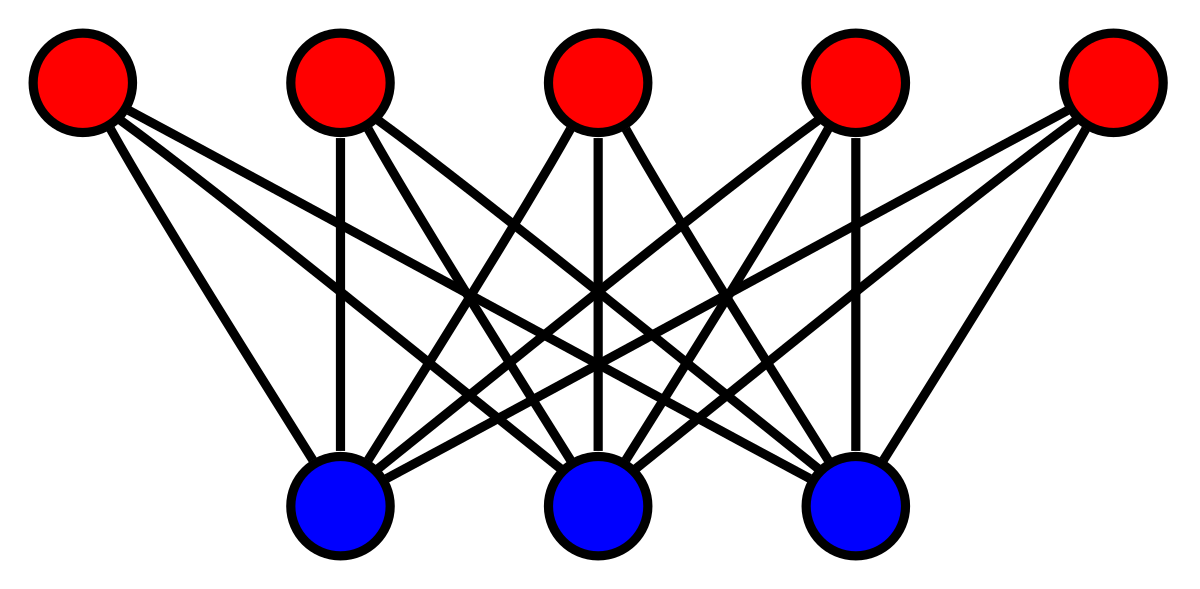
\includegraphics[scale = 0.2]{imagenes/K35.png}
		\end{center}
		\pause
		
		Probar que un grafo bipartito (no necesariamente completo) con un n\'umero impar de v\'ertices no contiene un circuito hamiltoniano.
	\end{minipage}
	
\end{frame}

\section{Planaridad}

\begin{frame}{Definiciones y Ejemplo}
	\begin{minipage}{\anchoPagina \textwidth}
		
		Un grafo $\mathcal{G}$ se dice planar si existe una representaci\'on en el plano donde sus aristas no se cruzan ni se cortan.
		
		Ejemplo: 
		\pause
		\begin{center}
			\includegraphics<2>[scale = 0.2]{imagenes/K4.png}
			\includegraphics<3->[scale = 0.35]{imagenes/K4-planar.png}			
			
			¿Es planar?
			

		\end{center}
		
		\pause
		\pause
		
% 		\textbf{Lema}: $\mathcal{G}$ es planar si y solo si todo bloque de $\mathcal{G}$ es planar.
		
	\end{minipage}	
\end{frame}

%\begin{frame}{F\'ormula de Euler}
%	\begin{minipage}{\anchoPagina \textwidth}
%		\textbf{Teorema}(F\'ormula caracter\'istica de Euler) : $|\mathbb{V}| + |\mathbb{R}| = |\mathbb{E}| + |\mathbb{C}| + 1$
%		\pause
		
%		$$ \text{V\'ertices} + \text{Regiones} = \text{Aristas} + \text{C.Conexas} + 1 $$
		
%		\pause
%		\textbf{Observaci\'on} $\mathcal{G}$ conexo y planar $\Rightarrow |\mathbb{V}| + |\mathbb{R}| = |\mathbb{E}| + 2$
		
%		\pause
%		Veamos por qu\'e vale este teorema \dots
%	\end{minipage}
%\end{frame}

\begin{frame}{Demostraci\'on}
	\begin{minipage}{\anchoPagina \textwidth}
		\textbf{Teorema}(F\'ormula caracter\'istica de Euler) : Si $\mathcal{G} = (\mathbb{V},\mathbb{E})$ es un grafo planar, entonces:  $|\mathbb{V}| + |\mathbb{R}| = |\mathbb{E}| + |\mathbb{C}| + 1$
		\pause
		
		$$ \text{V\'ertices} + \text{Regiones} = \text{Aristas} + \text{C.Conexas} + 1 $$
		\pause
		\begin{center}
			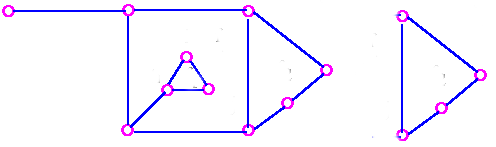
\includegraphics[scale = 0.4]{imagenes/euler.png}
		\end{center}
		
		\pause
		\textbf{Observaci\'on} $\mathcal{G}$ conexo y planar $\Rightarrow |\mathbb{V}| + |\mathbb{R}| = |\mathbb{E}| + 2$
		
		\pause
		Veamos por qu\'e vale este teorema \dots
	\end{minipage}
\end{frame}

\begin{frame}{Demostraci\'on}
	\begin{minipage}{\anchoPagina \textwidth}
		Supongamos que $\mathcal{G}$ tiene al menos una arista (un grafo sin aristas es trivialmente planar y cumple la ecuaci\'on, notar que la regi\'on exterior cuenta como tal)
		\pause
		
		Si $\mathcal{G}$ tiene al menos una arista, entonces hay dos casos:
		\pause
		\begin{enumerate}
			\item $\mathcal{G}$ es un \'arbol, entonces es planar. M\'as a\'un \pause $\Rightarrow n+1 = (n-1)+1+1$
			\pause
			\item $\mathcal{G}$ no es un \'arbol. Entonces podemos tomar $e \in \mathbb{E}$ que forme un ciclo. Luego, $e$ separa en dos regiones distintas. Entonces, si sacamos $e$ del grafo, por hip\'otesis inductiva en el grafo resultante, podemos afirmar que:
			$$ |\mathbb{V}| + (|\mathbb{R}| - 1) = (|\mathbb{E}|-1) + |\mathbb{C}| + 1  $$
			
			Por lo tanto \dots
			\pause
			$$ |\mathbb{V}| + |\mathbb{R}| = |\mathbb{E}| + |\mathbb{C}| + 1 $$
			
			que es lo que quer\'iamos probar.
				
		\end{enumerate}
	\end{minipage}
\end{frame}

\begin{frame}{Los grafos planares son ralos}
	\begin{minipage}{\anchoPagina \textwidth}
		Veamos un corolario interesante de la f\'ormula caracter\'istica de Euler.
		
		\textbf{Corolario}: $\mathcal{G}$ es conexo y planar con $|\mathbb{V}| \geq 3 \Rightarrow |\mathbb{E}| \leq 3|\mathbb{V}| - 6$
		
		\pause
		Idea: Notemos que se necesitan al menos 3 aristas para rodear una regi\'on. Si llamamos $r(i) = \# \text{aristas que rodean la regi\'on } i $.
		
		\pause
		Entonces, como cada arista limita con dos regiones (eventualmente la misma dos veces), la suma $\sum\limits_{i = 1}^{|\mathbb{R}|} \underbrace{r(i)}_{\geq 3} = 2|\mathbb{E}| \Rightarrow 2|\mathbb{E}| \geq \sum\limits_{i = 1}^{|\mathbb{R}|} 3 \Rightarrow |\mathbb{R}| \leq \frac{2}{3} |\mathbb{E}| $
		
		\pause 
		
		Como $|\mathbb{V}| + |\mathbb{R}| = |\mathbb{E}| + 2$ ($\mathcal{G}$ conexo) $\Rightarrow |\mathbb{R}| = |\mathbb{E}| + 2 - |\mathbb{V}| \leq \frac{2}{3} |\mathbb{E}| \Rightarrow \frac{|\mathbb{E}|}{3} \leq |\mathbb{V}| - 2 \Rightarrow \boxed{|\mathbb{E}| \leq 3|\mathbb{V}|-6} $
		
		\pause
		
		\textbf{Observaci\'on}:
		\begin{enumerate}
			\item $\mathcal{G}$ es conexo y planar $ \Rightarrow |\mathbb{E}| \in \mathcal{O}(|\mathbb{V}|) $, ¿C\'omo afecta esto a los algoritmos vistos?
			\item $K_5$ no es planar. Pues como es conexo, si fuese planar deber\'ia valer que: $\frac{5 \cdot 4}{2} \leq 3\cdot 5-6 \iff 10 <= 9$
		\end{enumerate}
	\end{minipage}
\end{frame}

\begin{frame}{Los grafos planares son ralos}
	\begin{minipage}{\anchoPagina \textwidth}
		\textbf{Corolario}: $\mathcal{G}$ conexo y planar sin tri\'angulos, entonces $|\mathbb{E}| \leq 2|\mathbb{V}| - 4$
		
		\pause ¿C\'omo demostramos esto? \pause ¡Igual que antes! solo que ahora podemos acotar a $r(i) \geq 4$.
		
		\textbf{Observaci\'on}: $K_{3,3}$ no es planar. Pues, es conexo y no tiene tri\'angulos (es bipartito, no tiene ciclos impares), sin embargo no cumple con el resultado del corolario.
		
% 		\pause
% 		\textbf{Mini ejercicio}: Probar que si $\mathcal{G}$ es un grafo planar, con circuitos todos ellos de longitud mayor o igual a $k$, podemos mejorar las desigualdades anteriores a: $\frac{(n-2)k}{k-2}$
	\end{minipage}
	
	 
	
\end{frame}

\begin{frame}{Caracterizaci\'on de grafos planares}
	\begin{minipage}{\anchoPagina \textwidth}
		 Decimos que un grafo $\mathcal{H}$ es una \textit{subdivisi\'on} de $\mathcal{G}$ si puedo obtener a $\mathcal{H}$ agregando v\'ertices en el medio de las aristas de $\mathcal{G}$.
		\pause
		\begin{center}
				\includegraphics<2>[scale = 0.1]{imagenes/subdivision-1.png}			\includegraphics<3->[scale = 0.1]{imagenes/subdivision-2.png}
		\end{center}
		\pause
		\pause
		
		\textbf{Teorema}(Kuratowski) Un grafo es planar si y solo si no contiene a una subdivisi\'on de $K_5$ ni $K_{3,3}$ como subgrafo.
	\end{minipage}
\end{frame}

\begin{frame}{S\'olidos Plat\'onicos}
	\begin{minipage}{\anchoPagina \textwidth}
		Decimos que un grafo es $\textit{plat\'onico}$ si cumple simult\'aneamente que:
		\begin{itemize}
			\item Es planar y conexo
			\item Es un grafo regular con grado mayor o igual a 3
			\item Cada regi\'on es rodeada por la misma cantidad de aristas en cualquier representaci\'on planar del grafo.
		\end{itemize}
		\textbf{Teorema}: Existen solo 5 \textit{grafos plat\'onicos}
		
		\pause
		\textbf{Demostraci\'on}: Llamemos $d$ al grado de los v\'ertices y $r$ a la cantidad de aristas que rodea cada regi\'on. Luego, de la definici\'on de grafo plat\'onico y usando la f\'ormula de la suma de los grados, obtenemos que:
		\begin{itemize}
			\item $2|\mathbb{E}| = d |\mathbb{V}|$
			\item $2|\mathbb{E}| = r |\mathbb{R}|$
		\end{itemize} 
		\pause
		
		Como es conexo y planar, por la f\'ormula caracter\'istica de Euler, tenemos que:
		$$|\mathbb{V}| + |\mathbb{R}| - 2 = |\mathbb{E}|  \Rightarrow \frac{2|\mathbb{E}|}{d} + \frac{2|\mathbb{E}|}{r} > |\mathbb{E}| \Rightarrow \frac{1}{d} + \frac{1}{r} > \frac{1}{2}$$
		\pause
		\begin{itemize}
			\item Como $d \geq 3 \Rightarrow \frac{1}{r} > \frac{1}{2} - \frac{1}{3} \Rightarrow  r < 6 \Rightarrow r \leq 5$
			\item Como $r \geq 3 \Rightarrow \frac{1}{d} > \frac{1}{2} - \frac{1}{3} \Rightarrow d < 6 \Rightarrow d \leq 5$
		\end{itemize} 
	\end{minipage}
	
\end{frame}

\begin{frame}{S\'olidos Plat\'onicos}
	\begin{minipage}{\anchoPagina \textwidth}
		Finalmente, podemos estudiar los 5 casos restantes a mano.
		\begin{enumerate}
			\item Si $d = 3, r = 3 \Rightarrow |\mathbb{V}| = 4, |\mathbb{R}| = 4$, obtenemos un \textit{tetraedro}.
			\item Si $d = 4, r = 3 \Rightarrow |\mathbb{V}| = 6, |\mathbb{R}| = 8$, obtenemos un \textit{octaedro}.
			\item Si $d = 5, r = 3 \Rightarrow |\mathbb{V}| = 12, |\mathbb{R}| = 20$, obtenemos un \textit{icosaedro}.
			\item Si $d = 3, r = 4 \Rightarrow |\mathbb{V}| = 8, |\mathbb{R}| = 6$, obtenemos un \textit{cubo}.
			\item Si $d = 3, r = 5 \Rightarrow |\mathbb{V}| = 20, |\mathbb{R}| = 12$, obtenemos un \textit{dodecaedro}. 
		\end{enumerate}
		\pause
		\begin{center}
			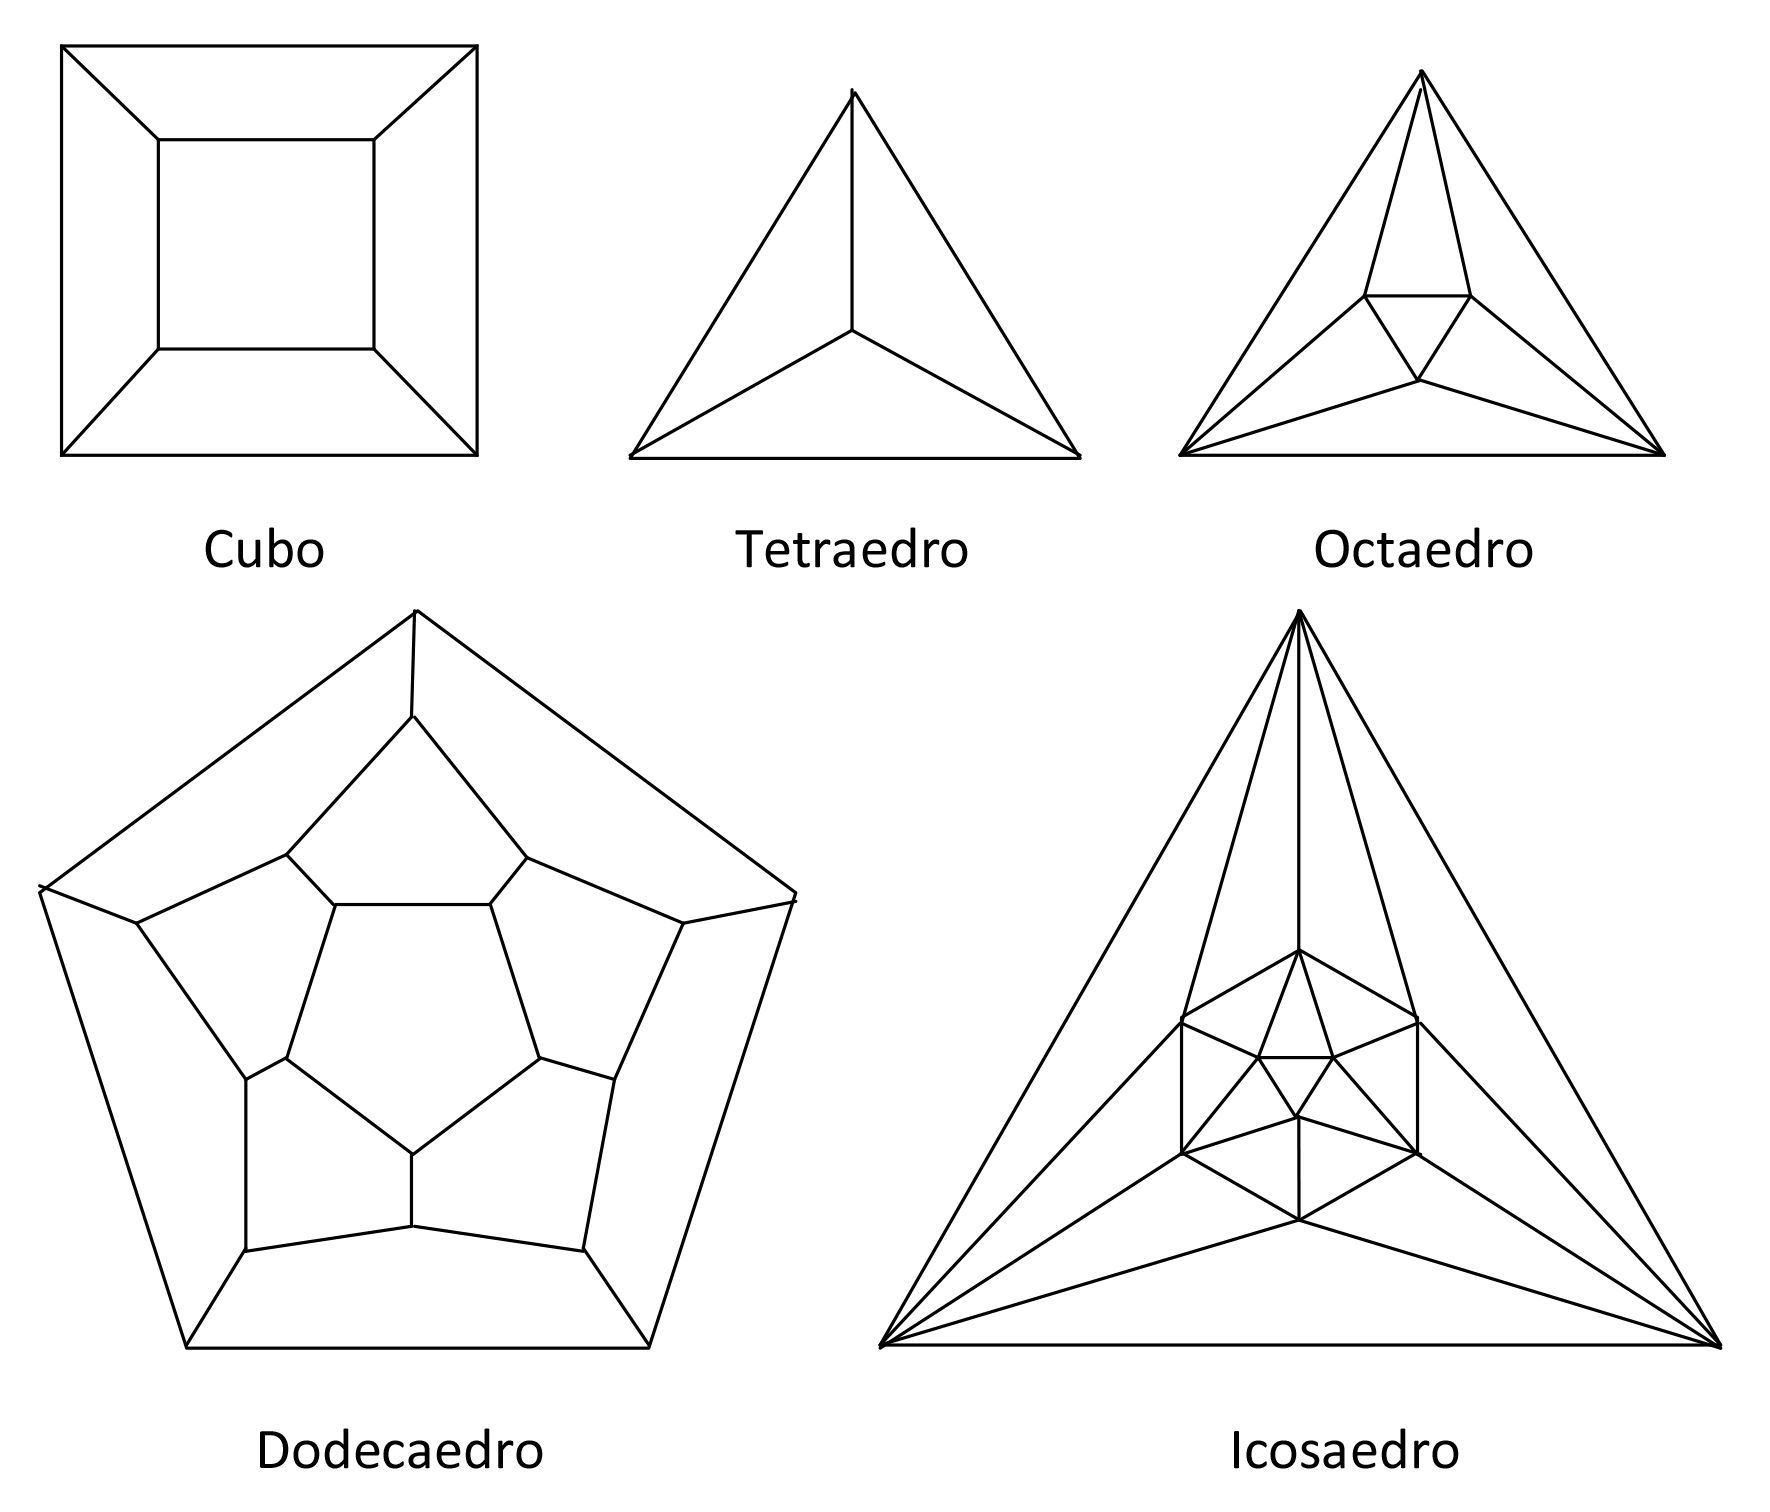
\includegraphics[scale = 0.09]{imagenes/grafos-platonicos}
		\end{center}
	\end{minipage}
\end{frame}

\begin{frame}{Grafo Dual}
	\begin{minipage}{\anchoPagina \textwidth}
		Dada una representaci\'on en el plano de un grafo se define su \textit{grafo dual} como el grafo que tiene:
		\begin{itemize}
			\item Un v\'ertice por cada regi\'on del grafo original
			\pause
			\item Una arista entre dos v\'ertices (regiones del grafo original) si las regiones son adyacentes (existe una arista con cada regi\'on a cada lado).
		\end{itemize}
		\pause
		\begin{center}
			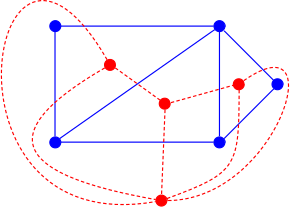
\includegraphics[scale = 0.3]{imagenes/dual.png}
		\end{center}
		\pause
		La dualidad no se preserva por isomofrfismo, esto podr\'ia ser intuitivo, dado que depende de la representaci\'on tomada del grafo.
	\end{minipage}
\end{frame}

\begin{frame}{Grafo Dual}
	\begin{minipage}{\anchoPagina \textwidth}
		La dualidad no se preserva por isomofrfismo, esto podr\'ia ser intuitivo, dado que depende de la representaci\'on tomada del grafo.
		
		\begin{center}
			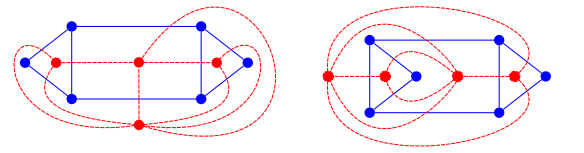
\includegraphics[scale = 0.5]{imagenes/dual-no-isomorfo.png}
		\end{center}
	\end{minipage}
\end{frame}


%\begin{frame}{Ejercicio}
%	
%	\pause
%	{\small 
%	El proceso de manufactura de una joya comienza con un pedazo de plata en bruto. La plata se tiene que \textit{tallar}, \textit{pulir}, \textit{agujerear} y \textit{marcar} de manera conveniente:
%	\begin{itemize}
%		\item Hay que tallarla antes que agujerearla.
%		\item Hay que pulirla antes que marcarla.
%	\end{itemize}
%	Adem\'as, cada proceso demora una cierta cantidad de tiempo.
%	\begin{itemize}
%		\item El proceso de tallado demora 1 unidad de tiempo.
%		\item El proceso de pulido demora 1 unidad de tiempo.
%		\item El proceso de marcado requiere de 2 unidades de tiempo si la pieza no est\'a tallada y 4 unidades de tiempo si la pieza est\'a tallada.
%		\item Agujerearla requiere de 3 unidades de tiempo si la pieza no est\'a pulida. Si la pieza est\'a pulida, pero no marcada, entonces agujerearla requiere de 5 unidades de tiempo. Por otro lado, si la pieza est\'a pulida y tambi\'en marcada, se requieren 7 unidades de tiempo para agujerearla.
%	\end{itemize}
	
%	Modelar el proceso mediante un grafo adecuado con el objetivo de realizar todos los procesos necesarios a la joya en cuesti\'on en el menor tiempo posible.
%	}
	
	
%\end{frame}




\end{document}

